\documentclass[a4paper]{article}
\author{Vincent Tran z3415372}
\usepackage{a4wide}
\usepackage{mathtools}
\usepackage{amsmath}
\usepackage {bsymb,b2latex}
\usepackage{graphicx}
\begin{document}

%%%%%%%%%%%%%%%%%%%%%%%%%%%%%%%%%%%%%%%%%%%%%%%%%%%%%%%%%%%%%%%%%%%%
\thispagestyle{empty}      % turn off page numbering
\begin{flushright}{\Large
System modelling and design \\[.3em]
Session 1, 2013}

\medskip
26 May 2013
\end{flushright}

\vfill
\fbox{\parbox{.9\textwidth}{%1347
\begin{center}
\huge\textbf{COMP2111 Assignment 3}\\
\bigskip\Large\textbf{Vincent Tran		z3415372	vtra143}
\end{center}
}}%1347
\vfill
\newpage
%%%%%%%%%%%%%%%%%%%%%%%%%%%%%%%%%%%%%%%%%%%%%%%%%%%%%%%%%%%%%%%%%%%%
\setcounter{page}{1}
%%%%%%%%%%%%%%%%%%%%%%%%%%%%%%%%%%%%%%%%%%%%%%%%%%%%%%%%%%%%%%%%%%%%
\section{Context and Sudokul}
Unfortuantely the only part of my model that you can play sudoku with AnimB. So I represented the grid as
\begin{align*}
 g \in  Row\cprod Col \pfun  Digits 
\end{align*}
which was what the spec wanted. I know some people put their definitions for the grid in the Context, but I thought that it didn't quite make sense to have it in the context. If you have the rules of the Sudoku game in the Context, they're defined by the axioms of the context. However, axioms are the foundations behind all of your calculations, such as commutativity of addition of natural numbers, which always hold true. While this is what you want, if an event breaks an axiom, you shouldn't be able to execute the event at all. The axioms define the scope of the machine, and if you have an event that could potentially invalidate your axioms, then your event is no longer in the scope of your machine.\\

The other three Invariants are just the rules of Sudoku. They look mindbogglingly long and complicated, but they aren't really. These two are the rules for having no number appear twice in the same column and row respectively.
\begin{align*}
& \forall  r \qdot  r \in  Row \limp  (\forall  c \qdot  c \in  Col \land  r \mapsto  c \in  dom(g)  \limp \\
&(\forall  c' \qdot  c' \in  Col\setminus \{ c\}  \land  r \mapsto  c' \in  dom(g) \limp  g(r \mapsto  c) \neq  g(r \mapsto  c')))
\end{align*}
\begin{align*}
 &\forall  c \qdot  c \in  Col \limp  (\forall  r \qdot  r \in  Row \land  r \mapsto  c \in  dom(g) \limp \\
&(\forall  r' \qdot  r' \in  Row\setminus \{ r\}  \land  r' \mapsto  c \in  dom(g) \limp  g(r \mapsto  c) \neq  g(r' \mapsto  c))) 
\end{align*}
They're basically the same thing, so I'm only going to explain one of them. In the first one, I scan all the rows r, and then as I'm scanning a row, I look at all the columns c and see if anything is in dom(g) (there's a number in that cell (r, c). I then look at all the other columns in that row, c' and compare the values there. In psuedocode it would look like:

\begin{verbatim}
for r in Row:
    for c in Col:
        if (r, c) in dom(g):
            for c' in Col\{c}:
                assert g(r, c) == g(r, c')
\end{verbatim}
The invariant to determine grids is a little bit different.
\begin{align*}
 &\forall  r, c \qdot  r \in  Row \land  c \in  Col \land  r \mapsto  c \in  dom(g) \limp  \\
&(\forall  r', c' \qdot  r' \in  Row \land  c' \in  Col \land  (r' = r \limp  c' \neq  c) \land  (c' = c \limp  r' \neq  r) \land \\
& (r- 1)/ 3 = (r'- 1)/ 3 \land  (c- 1)/ 3 = (c'- 1)/ 3 \land  r' \mapsto  c' \in  dom(g) \limp 
g(r \mapsto  c) \neq  g(r' \mapsto  c'))
\end{align*}
So basically you scan the entire grid and look for a cell (r, c) that has a number in it. We then look at every other cell (r', c') such that r' $\neq$ r and c' $\neq$ c, and we have check if (r, c) and (r', c') are in the same 3x3 square. Since I've made Row = 1$\upto$ 9 and Col = 1$\upto$9, to find out what 3x3 square (r, c) and (r', c') is in, we need to subtract 1 from the value and divide by 3. If that doesn't make sense, here's a diagram!
\centerline{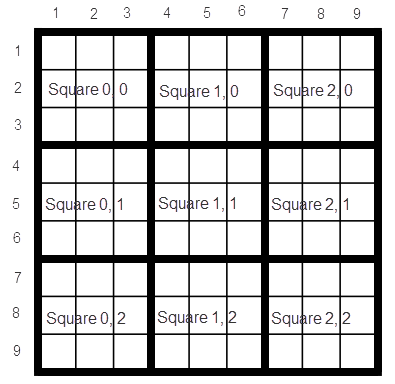
\includegraphics{sudokuGrid.png}}
Capiche? Yes? Good. Moving on.\\
So the \textit{setup} and \textit{fill} events are kind of boring. The guards are just the invariants copy and pasted, but I've replaced g with board for \textit{setup} and $g \ovl  \{ row \mapsto  col \mapsto  num\}$ for \textit{fill}. For the fill event, the point of replacing g with $g \ovl  \{ row \mapsto  col \mapsto  num\}$ is so that the guards will ensure that the post state of the event will not break the Invariants. The autoprovers somehow managed to discharge all the proof obligations straight off which is good :)\\
I had a little play around with AnimB and it got really annoying to check how many numbers where in the sudoku, so I added a variable numInSudoku to check how many numbers are in the sudoku. Play around with it. It's fun.

\section{Possibilities}
I'm not sure why, but AnimB asserts when I try to animate this even though I discharged all the proof obligations :(\\
So I modelled the possibilities as:
\begin{align*}
 p \in  Row\cprod Col \tfun  \pow(Digits)
\end{align*}
It's slightly different to the grid since you can't have a coordinate (r, c) that has an undefined number of possibilities. In an empty grid, each cell should have 1$\upto$9 as it's possibilities, not \textit{undefined}. The Invariants are more or less the same as the ones for the grid, only that g(r $\mapsto$ c) $\notin$ p(r $\mapsto$ c). \\
For the later parts of the assignment, I needed a way to access the cardinality of each possibility, but I couldn't figure out how to do it with just something like card(ran(p)), so I decided to introduce a new variable numPos which stored the number of possibilities of each cell. I think this ended up causing more problems than it fixed, but it ended up working out.\\
For INITIALISATION, I used the $\lambda$ function to initialise p and numPos. It's similar to anonymous functions in Python and C\# if you've used those.\\
With \textit{setup} and \textit{fill}, I've needed to update the possiblities in a completely verbose and ugly way. They're pretty much the same thing, so I'll only explain the \textit{setup} one.
\begin{align*}
&p, numPos :|  p' \in  Row\cprod Col \tfun  \pow(Digits) \land  numPos' \in  Row\cprod Col \tfun  \nat \land\\
&(\forall  r, c \qdot  r \in  Row \land  c \in  Col \land  r \mapsto  c \in  dom(board) \limp  p'(r \mapsto  c) = \{ board(r \mapsto  c)\}  \land \\
&(\forall  r' \qdot  r' \in  Row\setminus \{ r\}  \limp  p'(r' \mapsto  c) = p(r' \mapsto  c)\setminus \{ board(r \mapsto  c)\} ) \land\\
&(\forall  c' \qdot  c' \in  Col\setminus \{ c\}  \limp  p'(r \mapsto  c') = p(r \mapsto  c')\setminus \{ board(r \mapsto  c)\} ) \land \\
&(\forall  r', c' \qdot  r' \in  Row \land  c' \in  Col \land  (r' = r \limp  c' \neq  c) \land  (c' = c \limp  r' \neq  r) \land \\
&(r- 1)/ 3 = (r'- 1)/ 3 \land  (c- 1)/ 3 = (c'- 1)/ 3 \limp  p'(r' \mapsto  c') = p(r' \mapsto  c')\setminus \{ board(r \mapsto  c)\} )) \land \\
&(\forall  r, c \qdot  r \in  Row \land  c \in  Col \limp  numPos'(r \mapsto  c) = card(p'(r \mapsto  c)))
\end{align*}
Yay! It's also long and complicated and mindboggling! So let's break it down.
\begin{align*}
\forall  r, c \qdot  r \in  Row \land  c \in  Col \land  r \mapsto  c \in  dom(board) \limp  p'(r \mapsto  c) = \{ board(r \mapsto  c)\}
\end{align*}
You look at all the cells (r, c) that have a number in the cell and set the possibilities of (r, c) to a singleton set of the number board(r $\mapsto$ c). After that, we need to make sure the invariants hold, so we need to subtract board(r $\mapsto$ c) from the set of possibilities in every other cell in same row, column and square. That's what the next 4 lines are. It's important to note that p refers to the state before the action and p' refers to the state after. So in this assignment statement, p' becomes p and then some operations.\\
After updating all the possibilities, we set the values of numPos to card(p). The reason why this works is because the predicates occur in sequential order, not at the same time. So all of the possibilities of p have already updated before numPos gets updated.\\
You might've noticed that in the events, there's a guard that basically looks like the action, only with a  $\exists$ before everything. This was so that I could discharge FIS POs. Dodgy I know, but it works out because there won't be a situation where the guard disables the event and makes all the other POs go green (which can happen and is bad).

\section{Actions}
So I tried using data refinement here to eliminate EQL errors, so I had to declare new variables gr, pr, setupr and numPosr to replace g, p, setup and numPos respectively. It didn't quite work out as I wanted it to since instead of getting EQL POs, I got SIM and GRD POs which are just as equally hard/impossible to discharge. I couldn't figure out how to discharge these two POs because they involved proving things on the abstract variables which have disappeared. Because of this, there were no hypotheses that I could use the prove things about the abstract machine, hence the POs.\\
For autofill, I couldn't discharge some of the POs for gr (the rules for sudoku). Basically, I couldn't find a way to say that if a number is in the possibilities of a cell (r, c), putting a number $d \qdot d \in pr(r \mapsto c)$ in (r, c) will not break any of the Invariants. Other than that, everything else is proved.\\
I was a little bit confused as to the definition of the \textit{undo} event. The spec wasn't clear whether or not \textit{undo} remove the last move you did or that you could remove a number from a cell. I decided to go with the second one since it was significantly easier to prove - I tried the first one and it was too hard :(\\
The \textit{hint} event was the reason why I needed to add numPos into the system. The reason why I couldn't say card(ran(p)) is because the $ran(p) \le 10$, because the card(ran(p)) takes the cardinality of the entire range of p, not each individual cell.
\end{document}
